\section{Detection of Pores}\label{sec:pore_detection}

\begin{figure}
    \centering
    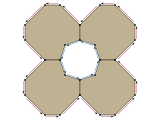
\includegraphics[width=\linewidth]{img/model_development/matrix_pore_detection}
    \caption{Principle of Detecting Pores in Multi-Particle Contacts}
    \label{fig:model_development/matrix_pore_detection}
\end{figure}

To be able to model the influence of a pore filled with fine-grained material on the large skeleton-particles, first the pores in a multi-particle contact must be found.
The procedure used is displayed in \cref{fig:model_development/matrix_pore_detection}.
This is done by choosing an arbitrary node and following its surface line to the next node (follow the arrows in the figure).
If a neck node is encountered, the procedure switches to the contacted particle and follows again the surface line (not in direction where the grain boundary is).
The procedure must always come back to the node where it has started, at which point the pore has been fully explored.
To find more pores, a new node, which has not been visited yet, is chosen arbitrarily and the procedure is repeated until all nodes have been visited.

In each particle system one or more closed line strings of this kind can be found.
The one always present is the outer surface of the whole system (the red line string in \cref{fig:model_development/matrix_pore_detection}).
Additional ones are pores which are surrounded by mutliple particles (the blue line string).
These two kinds can be distinguished in that way, the the one with the largest area must always be the outer surface.

The volume of a pore (area in 2D) is calculated with the shoelace formula as in \cref{eq:polygon-shoelace}, with $\Nodes$ as the set of nodes belonging to the pore's boundary.

\begin{equation}
    \Volume_{\Matrix} = \frac12 \sum_i^{\Nodes} \left( \Y_i + \Y_{i+1} \right) \left( \X_i - \X_{i+1} \right)
    \label{eq:polygon-shoelace}
\end{equation}
